\documentclass[10pt, conference, compsocconf]{IEEEtran}
\usepackage{graphics,color} % for pdf, bitmapped graphics files
\usepackage{subfigure}
\usepackage{rotating}
\usepackage{algorithmic}
\usepackage{comment}
\usepackage{algorithm,amssymb,url}
\usepackage{epsfig}
\usepackage[cmex10]{amsmath}
\usepackage{amsthm}
\usepackage{bm}
\usepackage{cite}
\usepackage{textcomp}
\usepackage{markdown}


\newboolean{showcomments}
\setboolean{showcomments}{true}

\ifthenelse{\boolean{showcomments}}
{ \newcommand{\mynote}[2]{
    \fbox{\bfseries\sffamily\scriptsize#1}
    {\small$\blacktriangleright$\textsf{\emph{#2}}$\blacktriangleleft$}}}
{\newcommand{\mynote}[2]{}}

%\newenvironment{todo}
%  {\begin{markdown}
%  }
%  { 
%  \end{markdown}
%  }


\newcommand{\cdu}[1]{\mynote{Corentin}{#1}}
% \newcommand{\todo}[1]{\mynote{TODO}{#1}}

\newcommand {\0} {\mathbf 0}
\newcommand {\1} {\mathbf 1}
\newcommand {\bt} {{\mathbf t}_c}
\newcommand {\bb} {{\mathbf b}}
\newcommand {\bx} {\mathbf x}
\newcommand {\eeq} {\end{equation}}
\newcommand {\barr} {\begin{array}}
\newcommand {\earr} {\end{array}}
\newcommand {\bear} {\begin{eqnarray}}
\newcommand {\wU} {\widehat U}
\newcommand {\namep} {Cloud4IoT\relax}
%\thispagestyle{plain}

\markdownSetup{
  renderers = {
    link     = {#1},        % Render a link as the link label.
    emphasis = {\emph{#1}}, % Render emphasis using `\emph`.
  }
}


\begin{document}

\title{Green IoT for developing countries}


\author{
Authors\\
FBK Create-Net, via alla Cascata 56/D, 38123 Trento, Italy.\\
\texttt{<xxx>@fbk.eu}
}

\maketitle

\begin{abstract}
- high development of IoT. IoT is also an enabler technology for IA.
- IoT as currently a low penetration in third world countries
- many external factors are disrupting traditional sectors in Africa.
- For instance, climate change is a big threat to agriculture sector.
- In the same time, sprawling urban development of African cities generate a lot of waste.
- IoT is needed to address those chalenges.
We show how IoT can meet African challenges.
Our solution is itself environmentaly conscious, with low impact hardware based on Arduino and LoRa.
We demonstrate the use of this technology in a use case where IoT is used to monitor water in Senegal.

\end{abstract}

\begin{IEEEkeywords}
IoT, Energy management, Cloud computing 
\end{IEEEkeywords}

\section{Introduction}
\label{intro}

\begin{markdown}
Intro outline:

- African market is growing very fast.
- In the same time, environmental problems are growing proportionally.
- IoT currently has low penetration in Africa, although the interest is growing steadily.
- The IoT has the potential to accompany and boost Africa's growth
- IoT can be used to improve energy and resource usage, and to improve waste disposal and recycling     

Motivation:

- African population adopted massively the mobile networks, with 93\% of the population having access to mobile phones. Landlines phones were never massively deployed on the continent.
- Similarly, Africa could jump into the era of open IoT and web platforms directly, skipping entirely the closed-silo industries. 
- The IoT hardware and software itself should be environmentally sustainable: low energy consumption, long life, recyclable
- Agricultural products are the main export and revenue in Africa.

\end{markdown}


ICT in developing countries has the potential to cut across traditional sectors: notable examples are the introduction of micro-health insurance and health-savings accounts through mobile devices; index-based crop insurance; crowd-sourcing to monitor and manage the delivery of public services.
These innovative applications recognize and leverage commonalities between sectors, blur traditional lines, and open up a new field of opportunities.
The opportunity for ICT intervention in developing countries is huge especially for IoT and big data: those technologies are promising a big wave of innovation for our daily life \cite{Sarkar2016,ITU2015}.

In this article, we present in Section \ref{iot} the new technologies and trends contributing in making IoT available at a much lower cost for worldwide adoption.
Then, we present in Section \ref{platform} the EU H2020 WAZIUP IoT platform targeting deployment of low-cost IoT and Big Data in developing countries, addressing the aforementioned major issues.
Section \ref{conclu} concludes the article.

\section{Challenges}
\label{iot}

\subsection{Societal challenges}

\begin{markdown}
Objectives:

- African market is expanding very fast. We believe IoT has a major role to play.
- Economic development should be made "colinear" with both environmental consciousness and human development. The objective is "sustainable growth".

Problems: 

- population in African cities is exploding.
     - Huge urbanisation problems appear, such as waste management.
     - Air polution
- Climate change is disrupting traditional agriculture
     - traditional method becomes obsolete (sowing at fixed times, traditional crop types etc.)
     - land can become polluted with excessive inputs
     - Agriculture is also very fragmented, with many small exploitations (85\% are less than 2 Ha)
     - Agriculture is also hindered by social and legal problems, such as the land ownership problem; and the conflict between official and traditional ruling.
- limited education: many farmers doesn't know IoT or ICT in general

Proposed solutions:

- On Agriculture:
     - Need to allow experts to provide analysis and recommendations, from remote
     - Farmers and advisers need to be trained to those new technologies
- On Urban development:
     - IoT-enabled urban informations, such as the level of wastes
     - Taylored for African cities, from the economic and social point of view: led by ONG, local/recycled material, right incentivization for the users


Constraints:

- Low cost and low power LoRa networks
- low power sensor nodes based on Arduino
- IoT should produce limited wastes, with a well defined hardware life cycle
- robustness of hardware
- low-tech solution such as SMS, USSD, Voice calls

Considerations:

- Mobile phone penetration is extremely high. In the same time, electrification and sanitation is low, especially in the countryside.
- Facebook is the number one social network in Africa. 

     
\end{markdown}
Mobile phone penetration: \footnote{https://www.gsmaintelligence.com/research/?file=3bc21ea879a5b217b64d62fa24c55bdf} \footnote{http://afrobarometer.org/publications/ad69-building-progress-infrastructure-development-still-major-challenge-africa}: 93\% of the continent population have access to mobile phones.

\subsection{Technical challenges}

\begin{markdown}
Hardware:

- rough environment: humidity in the box, sun (as with example of EGM buoy).
- sensor nodes can be stolen
- maintenance is difficult from remote: Battery problems, sensor nodes are removed from the field without notice etc.
- communication problems between gateway and nodes: plants growing can shield the antenna
- energy saving in the hardware: long battery duration

Software:

- Plug and play solution, without any configuration
- support intermittent connection
- access on mobile phone
- support of low-tech (SMS, USSD, voice calls)
- supports low data sampling rates, low reliability


\end{markdown}


\subsection{Requirements}

\section{Waziup platform}
\label{iot}

\subsection{Overview}

Insert here a picture of the whole platform (Hardware + software)

\subsection{IoT}

\begin{markdown}
Ideas:

- long battery duration with Arduinos
- Low cost and low power LoRa networks
- limited wastes, hardware life cycle
\end{markdown}
\subsection{Cloud Platform}

\begin{markdown}
outline:
- Architecture
- local Cloud
- support for social networks. 
\end{markdown}

We propose a Cloud platform in order to support our IoT deployments.

\begin{figure} 
\centering  
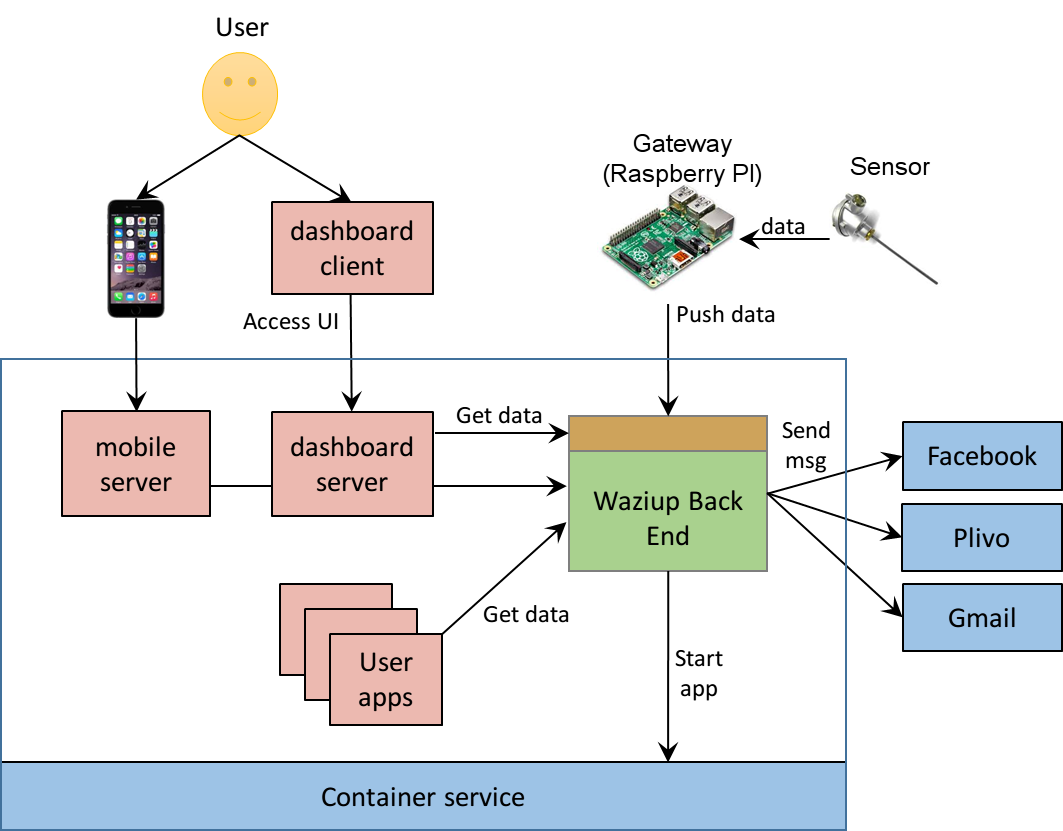
\includegraphics[width=.9\linewidth]{figs/CloudEnv}   
\caption{Cloud platform environment}   
\label{fig:cloudenv}  
\end{figure} 

\begin{figure} 
\centering  
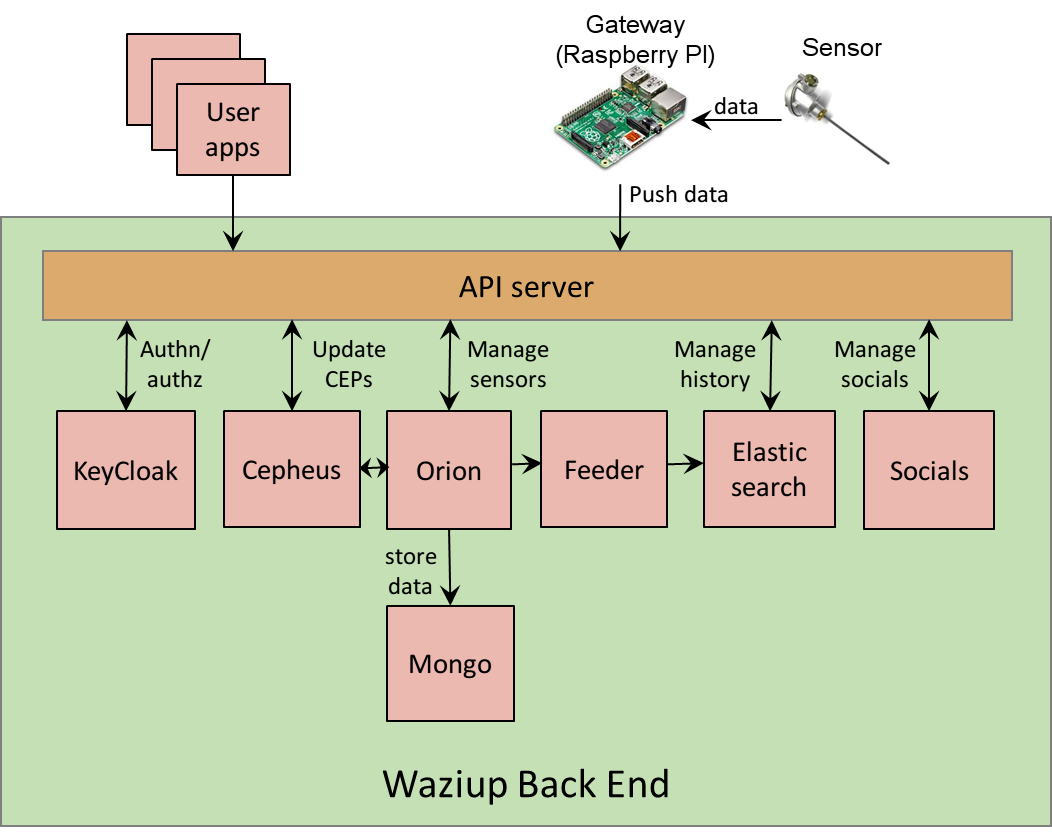
\includegraphics[width=.9\linewidth]{figs/BackEnd}   
\caption{Cloud platform backend}   
\label{fig:backend}  
\end{figure} 


\section{Use cases}

\subsection{Use case 1: water saving in Senegal}
\label{usecase}

We deploy IoT in order to save water in cultures.
\begin{markdown}
Outline:

- Introduction
- Scenarios
- Deployments

\end{markdown}


\subsection{Use case 2: Urban waste management in Togo}
\label{usecase}

IoT is used to reduce the Urban waste and promote recycling in Togo.
\begin{markdown}
Outline:

- Introduction
- Scenarios
- Deployments

\end{markdown}


\section{Related works}
\label{sota}

\paragraph{IoT in Africa}
There is very little penetration of IoT in Africa, as evidentiated in~\cite{Onyalo2015} and~\cite{Masinde2014}.
The authors of~\cite{Onyalo2015} provide a survey, country by country, of the undertaking of IoT.
They also document some of the challenges affecting adoption of IoT in the continent.
Africa has only 7\% of her households on the Internet; this is far behind the world’s figure of 41\%.
Given this lag in the baseline technology needed to implement Internet of Things, the author of~\cite{Masinde2014} advocate for a technological leap and an African-centric approaches to IoT.
Taking the case of a drought early warning and assets tracking systems, the author demonstrates that by innovatively incorporating the realities such as the prevalence of African indigenous knowledge on weather, unreliable communication, low-end mobile phone handsets, among others, a home-grown Internet of Things flavour has higher chance of succeeding.
An extensive report from Cisco~\cite{ITU2015} provides also many insights on the current use and potential of Internet of Things (IoT) technologies in tackling global development challenges, highlighting a number of specific instances where IoT interventions are helping to solve some of the world’s most pressing issues.


A deployment of a Wireless Sensor Network for precise irrigation in Malawi is presented in~\cite{Mafuta2013}.
For the system to be self-sustained in terms of power, the study used solar photovoltaic and rechargeable batteries to power all electrical devices.
The system incorporated a remote monitoring mechanism through a General Packet Radio Service modem to report soil temperature, soil moisture, WSN
link performance, and photovoltaic power levels. 
Irrigation valves were activated to water the field.
The paper give insights to develop a robust, fully automated, solar-powered, and low-cost irrigation system to suit the socioeconomic conditions of small scale farmers in developing countries.

The authors of~\cite{Dlodlo2015} provides a survey of possible IoT applications in South Africa and Zambia.
In particular, they identify examples of IoTs to mitigate the agricultural needs of these communities for the domains of crop farming, weather forecasting, wildlife management, forestry, livestock farming, market identification and rural financing.


\paragraph{IoT in Agriculture}
There is not a lot of literature on the specific topic of applying IoT in agriculture, and practically none went it comes to rural Africa.
In~\cite{Bing2012}, the author presents a work supporting the transition from traditional agriculture to modern agriculture in China.
They propose an agriculture intelligent system based on IOT for organic melon and fruit production. 
A number of new technologies are used, such as RFID and sensors.
They monitor temperature, humidity, light and $CO_2$ around the crops and use a small model on the fruits of growth process.
Always in China,~\cite{TongKe2013} uses Internet of things and RFID technologies to realize automatic control production of agriculture.

In~\cite{Dan2015}, the authors perform temperature control in greenhouse using Zigbee.
In~\cite{Hu2011a}, the authors elaborate a crop growth model.
The model is then embbeded in their IOT application system.
This allows them to make the system more intelligent and adaptive for the facility agriculture.
The authors of~\cite{Nakutis2015} and~\cite{Sarkar2016} proposes remote agriculture monitoring and process automation.
They are both based on gateway infrastructure and wireless connection.
The work in~\cite{Jayaraman2015} shows a semantically enhanced digital agriculture use case built with the OpenIoT platform.

In~\cite{Ilapakurti2015}, the authors uses IoT to check electronically on the vital signs of the cattles.
Their tool facilitates the day to day management of dairy activities.
It also provides forecastings allowing to handle weather related issues, cattle health and emergencies.

IoT is also deployed within the product supply chain, another key area of agriculture.
In~\cite{Han2014}, the authors builds a quantitative trust model to describe the trustworthiness of foods delivered in supply chains.
The Internet of Agricultural Things (AIoT), where the technologies of the Internet of Things are widely used in all of the phases in the agriculture industry, is proposed to resolve the food safety problem.
In order to provide a common model to describe and transmit the data in agriculture Internet of Things, \cite{Hu2011} proposes a specific ontology, while~\cite{Liu2014} uses a naming service to identify products.


With difference with the literature surveyed in this section, the proposed Waziup platform is a full IoT platform taylored entierly for African need and constraints.
In particular, it as application hosting capacities based on the PaaS paradigm, is resilient to disconnections and provides big data capacities.


\section{Conclusion}
\label{conclu}


\section*{Acknowledgment}
This research received funding from the European Union's H2020 Research and Innovation Action under grant agreement n. 688088 (project AGILE) and grant agreement n. 687607 (project WAZIUP).

\bibliographystyle{IEEEtran}
\bibliography{central-bibliography/bibliography}

\end{document}


